\section{Recommender Systems}

\subsection{Introduzione}

Un sistema di raccomandazione (Recommender System) \cite{RecommenderOverview} è un sistema software progettato per suggerire all'utente elementi di interesse, come ad esempio prodotti, servizi, informazioni o contenuti multimediali, in base alle preferenze e ai comportamenti passati dell'utente. I sistemi di raccomandazione sono ampiamente utilizzati in diversi contesti, come ad esempio il commercio elettronico, i social network, i servizi di streaming multimediale e le piattaforme di ricerca e informazione. I sistemi di raccomandazione sono utili per migliorare l'esperienza dell'utente, aumentare la soddisfazione e la fidelizzazione del cliente, e favorire la scoperta di nuovi contenuti e opportunità.
Questi sistemi sono basati su algoritmi di apprendimento automatico e intelligenza artificiale, che analizzano i dati relativi alle preferenze e ai comportamenti degli utenti, e generano raccomandazioni personalizzate in base a tali informazioni.\\

\begin{figure}[h!]
    \centering
    \begin{minipage}{0.2\textwidth}
        \centering
        
\includegraphics[width=\textwidth]{images/netflix.png}
    \end{minipage}\hfill
    \begin{minipage}{0.2\textwidth}
        \centering
        
\includegraphics[width=\textwidth]{images/amazon.png}
    \end{minipage}\hfill
    \begin{minipage}{0.2\textwidth}
        \centering
        
\includegraphics[width=\textwidth]{images/spotify.png}
    \end{minipage}\hfill
    \begin{minipage}{0.2\textwidth}
        \centering
        
\includegraphics[width=\textwidth]{images/tiktok.png}
    \end{minipage}
    \caption{Alcuni famose piattaforme che utilizzano sistemi di raccomandazione}
\end{figure}\


\noindent I sistemi di raccomandazione possono essere di diversi tipi, a seconda della tecnica utilizzata per generare le raccomandazioni.
\begin{itemize}
    \item \textbf{Collaborative filtering} \cite{CFRS}: generano raccomandazioni basandosi sulle valutazioni degli utenti per gli item
    \item \textbf{Content-based} \cite{Lops2011}: generano raccomandazioni basandosi sul contenuto degli item e sulle preferenze dell'utente
    \item \textbf{Knowledge-aware} \cite{KnowledgeAware}: l'idea è quella di fondere informazioni provenienti da diverse fonti di conoscenza.
    \item \textbf{Approci ibridi}: combinano le tecniche precedenti
\end{itemize}



\begin{table}[H]
    \centering
    \footnotesize
    \setlength\tabcolsep{0pt}
    \begin{tabularx}{\textwidth}{|X|X|}
        \hline
        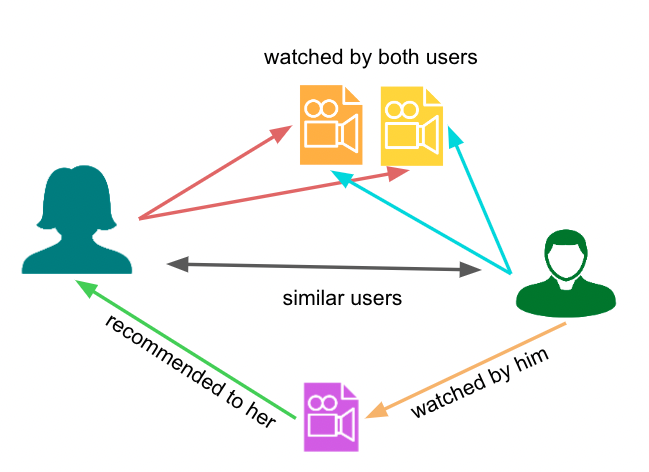
\includegraphics[width=\linewidth, trim=0 0 0 0]{images/cfRecSys.png} &
        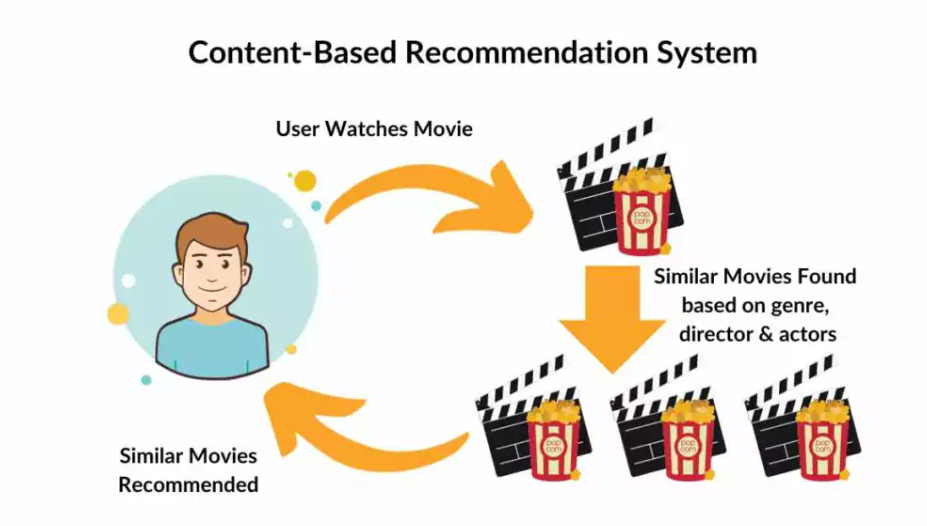
\includegraphics[width=\linewidth, trim=0 0 0 0]{images/contentbased.png} \\
        \hline
        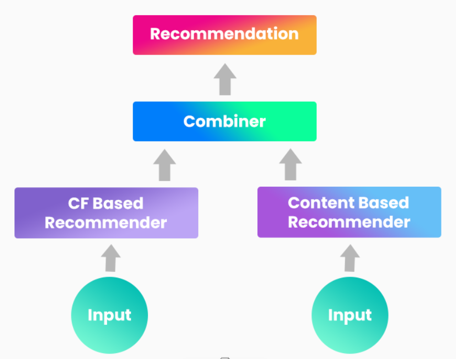
\includegraphics[width=\linewidth, trim=0 0 0 0]{images/hybridRecSys.png} &
        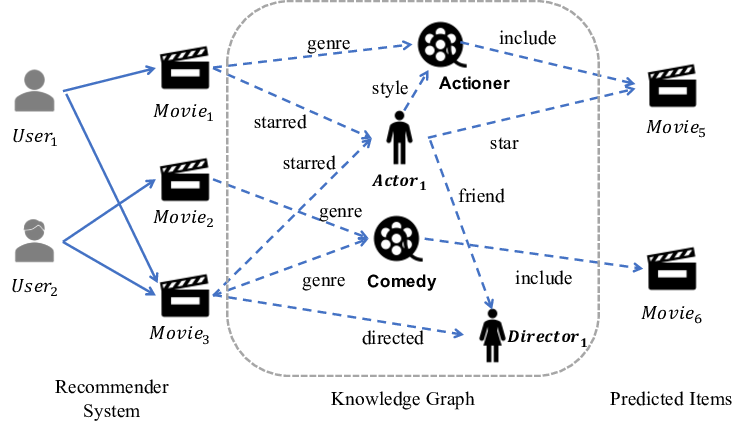
\includegraphics[width=\linewidth, trim=0 0 0 0]{images/knowledge.png} \\
        \hline
    \end{tabularx}
    \caption{Tipi di Recommender Systems}
\end{table}


\noindent Per valutare le prestazioni di un sistema di raccomandazione si possono utilizzare diverse metriche che è possibile riassumere nelle seguenti categorie:
\begin{itemize}    
    \item \textbf{Classification metrics}: queste metriche valutano la capacità del sistema di classificare correttamente gli elementi in base alle preferenze dell'utente. Alcune delle metriche più comuni sono l'accuracy, la precision, il recall e l'F1-score.

    \item \textbf{Accuracy metrics}: queste metriche valutano la precisione e l'accuratezza delle raccomandazioni generate dal sistema. Alcune delle metriche più comuni sono l'RMSE (Root Mean Squared Error) e il MAE (Mean Absolute Error).
    \item \textbf{Ranking metrics}: queste metriche valutano la qualità dell'ordinamento delle raccomandazioni generate dal sistema. Alcune delle metriche più comuni sono il coefficiente di correlazione di Kendall Tau, il coefficiente di correlazione di Spearman, l'NDCG (Normalized Discounted Cumulative Gain).
    \item \textbf{Diversity metrics}: queste metriche valutano la diversità delle raccomandazioni generate dal sistema. Alcune delle metriche più comuni sono la diversità delle raccomandazioni e la novità delle raccomandazioni.
    \item \textbf{Coverage metrics}: queste metriche valutano la copertura degli elementi raccomandati dal sistema.
\end{itemize}    

\noindent Alcuni tipici problemi che si possono incontrare nella progettazione e nell'implementazione di un sistema di raccomandazione sono:
\begin{itemize}
    \item \textbf{Cold start problem} \cite{ColdStart}: il problema del cold start si verifica quando un nuovo utente o un nuovo elemento si registra nel sistema e non ci sono dati sufficienti per generare raccomandazioni personalizzate.
    \item \textbf{Data sparsity problem} \cite{DataSparsity}: nella maggior parte delle reali applicazioni il numero di item è molto maggiore del numero di item valutati da ciascun utente. Questo porta a una matrice di valutazioni molto sparsa, che rende difficile la generazione di raccomandazioni accurate
    \item \textbf{Vulnerabilità agli attacchi} \cite{Attacchi} : i sistemi di raccomandazione possono essere vulnerabili a diversi tipi di attacchi, come ad esempio le recensioni fake (tipico problema degli e-commerce)
\end{itemize}

\subsection{Collaborative Filtering}
I sistemi di raccomandazione collaborative filtering generano raccomandazioni/filtrano i contenuti basandosi sull' "opinione" di altri utenti\cite{CFRS}.\\ Con il termine utente ci si riferisce a qualsiasi individuo che inserisca delle valutazioni per gli item presenti nel sistema\cite{CFRS}. \\ Gli item sono gli oggetti che vengono raccomandati agli utenti (es. film, libri, prodotti, etc.)\cite{CFRS}.\\
L'idea alla base del collaborative filtering è creare una matrice di valutazioni utente-item, in cui ogni cella della matrice rappresenta la valutazione di un utente per un item.\\ Le valutazioni sono in genere numeriche, e possono essere espresse in termini di rating (es. da 1 a 5 stelle) o di preferenze (es. like/dislike).\cite{CFRS}\\
Esistono principalmente due tipi di collaborative filtering:
\begin{itemize}
    \item \textbf{User-based collaborative filtering}: in questo approccio, le raccomandazioni vengono generate confrontando le preferenze dell'utente con quelle degli altri utenti \cite{CFRS}. In particolare, si calcola la similarità tra l'utente target e gli altri utenti, e si generano raccomandazioni basate sulle preferenze degli utenti più simili all'utente target. Due utenti sono ritenuti simili se hanno uno stile di valutazione simile per gli item (cioè valutano gli stessi item in modo simile)
    \item \textbf{Item-based collaborative filtering}: in questo approccio, le raccomandazioni vengono generate confrontando le preferenze degli utenti per gli item. In particolare, si calcola la similarità tra gli item, e si generano raccomandazioni basate sugli item più simili a quelli valutati positivamente dall'utente target. Due item sono ritenuti simili se vengono valutati in modo simile dagli stessi utenti\cite{ItemBased}.
\end{itemize}
I principali vantaggi del collaborative filtering sono la sua semplicità e la sua capacità di generare raccomandazioni personalizzate senza la necessità di dover conoscere le caratteristiche degli item (es. la durata di un film, il genere di un libro, etc.). Tuttavia, il collaborative filtering può soffrire di problemi come il cold start (per un nuovo utente e per un nuovo item), la vulnerabilità agli attacchi come le recensioni fake e la scarsa spiegaibilità delle raccomandazioni generate.\\


\begin{table}[H]
    \centering
    \begin{tabular}{|c|c|c|c|c|}
        \hline
        & Item 1 & Item 2 & Item 3 & Item 4 \\
        \hline
        User 1 & 5 & 4 & 0 & 0 \\ \hline
        User 2 & 0 & 0 & 3 & 4 \\ \hline
        User 3 & 0 & 0 & 0 & 0 \\ \hline
        User 4 & 0 & 0 & 0 & 0 \\
        \hline
    \end{tabular}
    \caption{Esempio di matrice utente-item}
\end{table}


\subsubsection{User-based collaborative filtering}
Ad oggi esistono diversi algoritmi per implementare il collaborative filtering user-based. Di seguito viene presentanto uno degli algoritmi più semplici \cite{CFRS}.\\
Dato l'utente target $u$, definiamo \textit{vicini} di $u$ un numero $n$ di utenti che hanno valutato in modo simile a $u$. Questi costituiscono il \textit{neighborhood} \textbf{N} (vicinato) di $u$.\\
L'idea alla base per predirre la valutazione di un item $i$ per l'utente $u$ è calcolare la media delle valutazioni degli item da parte dei vicini di $u$ per l'item $i$.\\
La formula per calcolare la predizione è la seguente:
\begin{equation}
    pred(u,i) = \frac{\sum_{n \in N} r_{ni}}{n}
\end{equation}
Questo approccio però non tiene conto che non tutti gli utenti sono ugualmente simili a $u$. Per ovviare a questo problema si può utilizzare una versione pesata della formula precedente, dove il peso è dato dalla similarità tra l'utente $u$ e l'utente $n$.
\begin{equation}
    pred(u,i) = \frac{\sum_{n \in N} r_{ni} \cdot sim(u,n)}{\sum_{n \in N} sim(u,n)}
\end{equation}
Poichè le valutazioni avvengono su scale numeriche la media pesata non dovrebbe essere calcolata tenendo conto solo della valutazione data all'item $i$ dall'utente $n$, ma anche della differenza tra la valutazione data da $n$ e la media delle valutazioni di $n$. Questo perchè un utente che valuta sempre in modo molto alto o molto basso non è molto affidabile e dunque bisogna tener conto dello stile di valutazione dell'utente.
\begin{equation}
    pred(u,i) = \bar{r_u} + \frac{\sum_{n \in N} (r_{ni} - \bar{r_n}) \cdot sim(u,n)}{\sum_{n \in N} sim(u,n)}
\end{equation}
Per il calcolo della similarità tra gli utenti si possono usare diverse metriche, come per esempio il coefficiente di correlazione di Pearson \cite{Pearson}:
\begin{equation}
    sim(u,n) = \frac{\sum_{i \in I} (r_{ui} - \bar{r_u}) \cdot (r_{ni} - \bar{r_n})}{\sqrt{\sum_{i \in I} (r_{ui} - \bar{r_u})^2} \cdot \sqrt{\sum_{i \in I} (r_{ni} - \bar{r_n})^2}}
\end{equation}

\subsubsection{Item-based collaborative filtering}

Anche per il collaborative filtering item-based esistono diversi algoritmi per implementarlo. Di seguito viene presentato uno degli algoritmi più semplici \cite{ItemBased}.\\
Data $u$ l'utente target e $i$ l'item target, l'idea alla base di questo approccio è calcolare la similarità tra l'item $i$ e gli altri item valutati da $u$.\\
La formula per calcolare la predizione è la seguente:
\begin{equation}
    pred(u,i) = \frac{\sum_{j \in I} r_{uj} \cdot sim(i,j)}{\sum_{j \in I} sim(i,j)}
\end{equation}
dove la similarità tra due item $i$ e $j$ può essere calcolata utilizzando diverse metriche, come per esempio la similarità coseno aggiustata \cite{CosineAdjustedSim}:
\begin{equation}
    sim(i,j) = \frac{\sum_{u \in U} (r_{ui} - \bar{r_u}) \cdot (r_{uj} - \bar{r_u})}{\sqrt{\sum_{u \in U} (r_{ui} - \bar{r_u})^2} \cdot \sqrt{\sum_{u \in U} (r_{uj} - \bar{r_u})^2}}
\end{equation}

\subsection{Content-based}
I sistemi di raccomandazione content-based generano raccomandazioni basate sul contenuto degli item (descritti da testo o mediante feature) e sulle valutazioni passate dell'utente \cite{Lops2011}.\\
Un sistema di raccomandazione content-based è composto da tre componenti principali \cite{Lops2011}:
\begin{itemize}
    \item \textbf{Profile learner}: Questa componente colleziona i dati relativi alle preferenze dell'utente e cerca di generalizzarle per creare un profilo dell'utente. Spesso questa generalizzazione avviene mediante tecniche di apprendimento automatico.
    \item \textbf{Content analyzer}: Questa componente ha come scopo quello di estrarre le caratteristiche degli item. Quando le descrizioni non sono strutturate (es. testo) è necessaria una fase di pre-processing per estrarre le caratteristiche rilevanti.
    \item \textbf{Filtering Component}: Questa componente ha come scopo quello di generare raccomandazioni personalizzate in base al profilo dell'utente e alle caratteristiche degli item. In particolare, si calcola la somiglianza tra il profilo dell'utente e le caratteristiche degli item, e si generano raccomandazioni basate su questa somiglianza.
\end{itemize}
\begin{figure}[H]
    \centering
    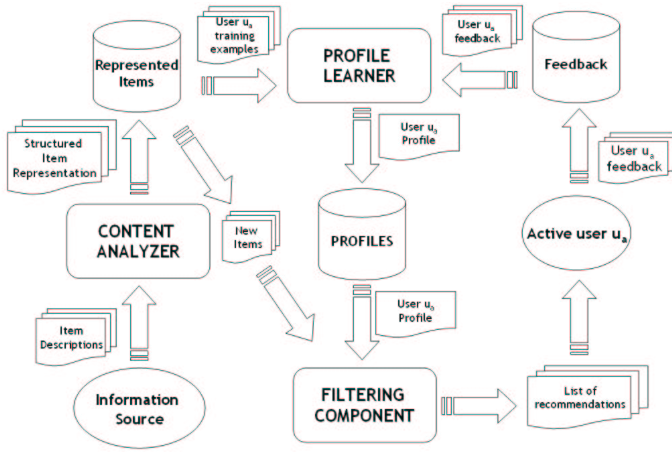
\includegraphics[scale=0.5]{images/contentBasedElementi.png}
    \caption{Architettura di un sistema di raccomandazione content-based}
\end{figure}

\noindent Per costuire e aggiornare il profilo dell'utente vengono raccolte le sue valutazioni. Queste possono essere esplicite quando all'utente viene richiesto di esprimere un giudizio in modo attivo (es. rating da 1 a 5 stelle, like/dislike) o implicite quando il sistema deduce le preferenze dell'utente in modo passivo (es. click, tempo trascorso su una pagina, etc.). Il vantaggio del feedback esplicito risiede nella sua semplicità, ma scale di valutazione molto grandi (es. da 1 a 100) possono portare a un carico cognitivo elevato per l'utente. Il feedback implicito non comporta alcuno sforzo da parte dell'utente, ma non è in grado di catturare le preferenze dell'utente in modo accurato.\cite{Lops2011}\\
Nei sistemi più recenti gli item sono descritti mediante testo, dunque una rappresentazione non strutturata. Per estrarre le feature rilevanti da un testo si possono utilizzare tecniche di IR (Information Retrieval) come ad esempio il TF-IDF (Term Frequency-Inverse Document Frequency).\\
Siano dati una collezione di documenti $D = \{d_1, d_2, ..., d_n\}$ e un dizionario di termini $T = \{t_1, t_2, ..., t_m\}$, ogni documento $d_i$ può essere rappresentato come un vettore di pesi $V_i = \{v_{i1}, v_{i2}, ..., v_{im}\}$, dove $v_{ij}$ rappresenta il peso del termine $t_j$ nel documento $d_i$.\\
Il calcolo del TF-IDF segue i seguenti principi \cite{TFIDF}:
\begin{itemize}
    \item i termini rari nella collezione portano più informazione rispetto ai termini comuni
    \item termini che compaiono più volte in un documento sono più rilevanti rispetto ai termini che compaiono poche volte nello stesso
    \item i documenti più lunghi non devono avere un peso maggiore rispetto ai documenti più corti
\end{itemize}
Il calcolo del TF-IDF è il prodotto tra il TF (Term Frequency) e l'IDF (Inverse Document Frequency):
\begin{equation}
    TF-IDF(t,d,D) = TF(t,d) \cdot IDF(t,D)
\end{equation}
Il TF è il numero di volte che il termine $t$ appare nel documento $d$:
\begin{equation}
    TF(t,d) = \frac{f_{t,d}}{\sum_{t' \in d} f_{t',d}}
\end{equation}
L'IDF è l'inverso della frequenza del termine $t$ nella collezione di documenti $D$ e viene calcolato come segue:
\begin{equation}
    IDF(t,D) = \log \frac{|D|}{|\{d \in D : t \in d\}|}
\end{equation}
Per calcolare la similarità tra due documenti $d_i$ e $d_j$ si può utilizzare la similarità coseno \cite{CosineSim}:
\begin{equation}
    sim(d_i,d_j) = \frac{V_i \cdot V_j}{||V_i|| \cdot ||V_j||}
\end{equation}
Nei sistemi di raccomandazione basati sui contenuti che si affidano al modello vettoriale (VSM), sia i profili degli utenti sia gli articoli sono rappresentati come vettori ponderati di termini. Le previsioni dell'interesse di un utente in un particolare articolo possono essere derivate calcolando la similarità coseno.
Le feature testuali però possono presentare diversi problemi:
\begin{itemize}
    \item \textbf{Polisemia}: una parola può avere diversi significati
    \item \textbf{Sinonimia}: diversi termini possono avere lo stesso significato
\end{itemize}
Uno degli approci più utilizzati per risolvere questo problema è quello dell'analisi semantica. L'idea è di utilizzare delle basi di conoscenza (come per esempio delle ontologie) per estrarre una "rappresentazione semantica" degli item e costruire/aggiornare il profilo dell'utente in base a questa rappresentazione\cite{Lops2011}.\\

\noindent I principali vantaggi dell'approccio content-based sono l'indipendenza dal comportamento degli altri utenti e la capacità di generare raccomandazioni personalizzate anche per nuovi item. Inoltre c'è una maggiore spiegabilità delle raccomandazioni generate. Tuttavia, i sistemi di raccomandazione content-based possono soffrire di problemi come la scarsa diversità delle raccomandazioni e la difficoltà di estrarre le caratteristiche rilevanti degli item. Rimane comunque il problema di cold-start per un nuovo utente\cite{Lops2011}.


\subsection{Knowledge-aware}
I sistemi di raccomandazione knowledge-aware generano raccomandazioni basandosi su conoscenza esterna\cite{KnowledgeAware}.Un esempio di conoscenza esterna sono i knowledge-graph: grafi di dati intenti ad accumulare e trasmettere conoscenze del mondo reale, i cui nodi rappresentano entità di interesse e i cui archi rappresentano potenzialmente diverse relazioni tra queste entità\cite{KnowledgeGraph}.Un grafo dunque può essere rappresentato come un insieme di triple RDF (soggetto, predicato, oggetto) dove soggetto e oggetto sono nodi del grafo, mentre il predicato è un arco.
\begin{figure}[H]
    \centering
    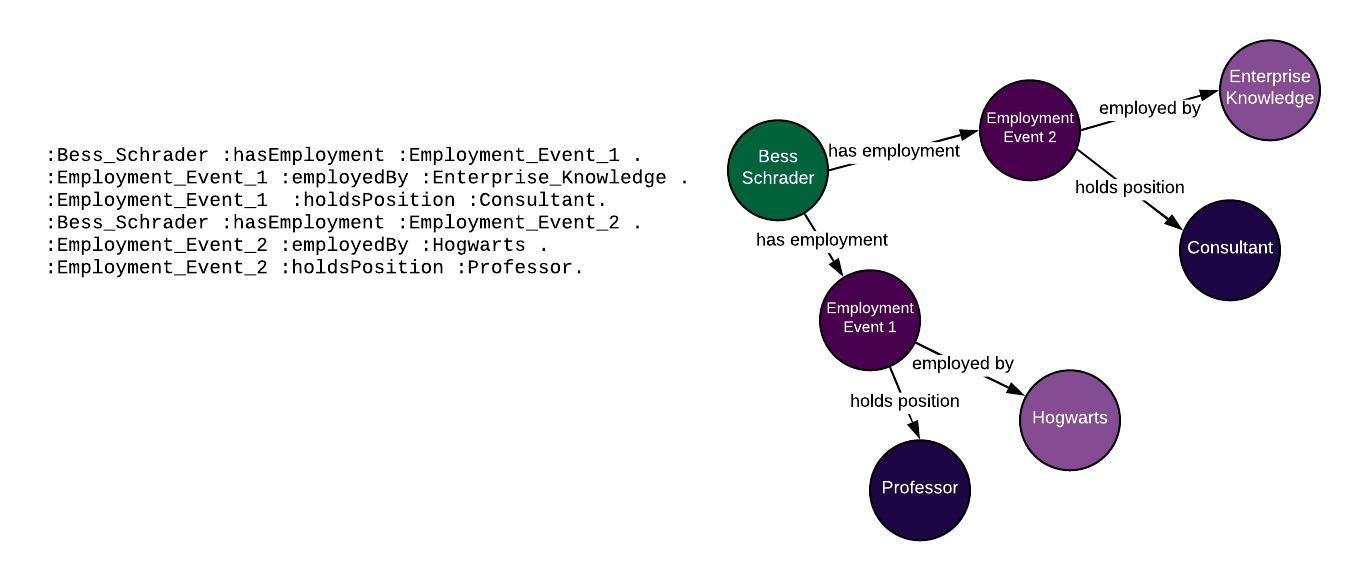
\includegraphics[scale=0.5]{images/graph.png}
    \caption{Esempio di knowledge-graph e triple RDF}
\end{figure} 
\noindent I sistemi di raccomandazione knowledge-aware utilizzano i knowledge-graph per rappresentare le caratteristiche degli item e le preferenze dell'utente, e generare raccomandazioni basate su questa rappresentazione. Possono esere seguiti diversi approcci  \cite{NeuroSimb}:
\begin{itemize}
    \item \textbf{Neural Reasoning}: lo scopo di questo metodo è quello di generare degli embedding per nodi ed archi del grafo in modo tale che questi mantengano la loro semantica anche nella loro rappresentazione vettoriale. Ottenuti i knowledge graph embedding \cite{KGEmbedd}, possono essere applicati diversi modelli di machine learning (tra cui anche reti neurali) per risolvere un problema di Knowledge Graph Completion (trovare nuove relazioni tra nodi del grafo usando il ragionamento logico).
    \item \textbf{Symbolic Reasoning}: l’idea di questo metodo è quella di dedurre un insieme di regole logiche a partire da un knowledge graph, fatto ciò le regole ottenute possono essere utilizzate per fare inferenza e scoprire nuove relazioni tra entità.
    \item \textbf{Neuro-symbolic Reasoning}: questo metodo combina i due metodi precedenti. Si generano degli embedding per gli elementi del grafo e, a partire da questi, un set di regole simboliche.
\end{itemize}

\noindent I principale vantaggio dei sistemi di raccomandazione knowledge-aware l'assenza del problema di cold-start. Tuttavia, i sistemi di raccomandazione knowledge-aware possono soffrire di problemi come la scarsa spiegabilità delle raccomandazioni generate e la difficoltà di rappresentare la conoscenza semantica in modo accurato e completo. Inoltre, i sistemi di raccomandazione knowledge-aware possono richiedere una quantità significativa di risorse computazionali per generare raccomandazioni accurate e rilevanti.\\

\subsection{Modelli di raccomandazione a stato dell'arte}
Negli ultimi anni, sono stati proposti diversi modelli di raccomandazione basati su diverse tecniche, che hanno ottenuto risultati molto promettenti in termini di accuratezza e prestazioni. Questi modelli sono chiamati a stato dell'arte (\textbf{SOTA}) per l'implementazione di sistemi di raccomandazione. Alcuni esempi di modelli di raccomandazione a stato dell'arte sono:
\begin{itemize}
    \item \textbf{ItemKNN} \cite{ItemKNN}: ItemKNN è un modello di raccomandazione basato su collaborative filtering item-based. In particolare, ItemKNN calcola la similarità tra gli item e genera raccomandazioni basate sugli item più simili a quelli valutati positivamente dall'utente target.
    \item \textbf{BPR} \cite{BPR}: BPR (Bayesian Personalized Ranking) è un modello di raccomandazione basato su collaborative filtering user-based. In particolare, BPR calcola la similarità tra gli utenti e genera raccomandazioni basate sugli utenti più simili all'utente target.
    \item \textbf{CFKG} \cite{CFKG}: CFKG è un modello di raccomandazione basato su collaborative filtering e knowledge-aware. In particolare, CFKG utilizza i knowledge-graph per rappresentare le caratteristiche degli item e le preferenze dell'utente, e genera raccomandazioni basate su questa rappresentazione.
    \item \textbf{CKE} \cite{CKE}: CKE (Collaborative Knowledge Embedding) è un modello di raccomandazione basato su collaborative filtering e knowledge-aware. In particolare, CKE utilizza tecniche di embedding per rappresentare le caratteristiche degli item e le preferenze dell'utente, e genera raccomandazioni basate su questa rappresentazione.
    \item \textbf{DMF} \cite{DMF}: DMF (Deep Matrix Factorization) è un modello di raccomandazione basato su deep learning. In particolare, DMF utilizza tecniche di deep learning per apprendere le rappresentazioni latenti degli item e degli utenti, e genera raccomandazioni basate su queste rappresentazioni.
    \item \textbf{KGCN} \cite{KGCN}: KGCN (Knowledge Graph Convolutional Networks) è un modello di raccomandazione basato su deep learning e knowledge-aware. In particolare, KGCN utilizza tecniche di deep learning e convolutional neural networks per apprendere le rappresentazioni degli item e degli utenti a partire dai knowledge-graph, e genera raccomandazioni basate su queste rappresentazioni.
    \item \textbf{KGNNLS} \cite{KGNNLS}: KGNNLS (Knowledge Graph Neural Network with Latent Space) è un modello di raccomandazione basato su deep learning e knowledge-aware. In particolare, KGNNLS utilizza tecniche di deep learning e neural networks per apprendere le rappresentazioni degli item e degli utenti a partire dai knowledge-graph, e genera raccomandazioni basate su queste rappresentazioni.
    \item \textbf{LINE} \cite{LINE}: LINE (Large-scale Information Network Embedding) è un modello di raccomandazione basato su deep learning e knowledge-aware. In particolare, LINE utilizza tecniche di deep learning e neural networks per apprendere le rappresentazioni degli item e degli utenti a partire dai knowledge-graph, e genera raccomandazioni basate su queste rappresentazioni.
    \item \textbf{MultiDAE} \cite{MultiDAE}: MultiDAE è un modello di raccomandazione basato su deep learning. In particolare, MultiDAE utilizza tecniche di deep learning e variational autoencoders per apprendere le rappresentazioni latenti degli item e degli utenti, e genera raccomandazioni basate su queste rappresentazioni.
    \item \textbf{LightGCN} \cite{LightGCN}: LightGCN è un modello di raccomandazione basato su deep learning. In particolare, LightGCN utilizza tecniche di deep learning e graph convolutional networks per apprendere le rappresentazioni latenti degli item e degli utenti, e genera raccomandazioni basate su queste rappresentazioni.
    \item \textbf{NGCF} \cite{NGCF}: NGCF (Neural Graph Collaborative Filtering) è un modello di raccomandazione basato su deep learning. In particolare, NGCF utilizza tecniche di deep learning e graph convolutional networks per apprendere le rappresentazioni latenti degli item e degli utenti, e genera raccomandazioni basate su queste rappresentazioni.
    \item \textbf{DGCF} \cite{DGCF}: DGCF (Dual Graph Collaborative Filtering) è un modello di raccomandazione basato su deep learning. In particolare, DGCF utilizza tecniche di deep learning e graph convolutional networks per apprendere le rappresentazioni latenti degli item e degli utenti, e genera raccomandazioni basate su queste rappresentazioni.
\end{itemize}


\noindent Ovviamente ci sono tanti altri modelli di raccomandazione a stato dell'arte, ma questi sono solo alcuni esempi.\\
I progettisti di Recommender Systems spesso prendono spunto da questi modelli per creare nuovi modelli che possano adattarsi meglio alle esigenze specifiche del problema che si vuole risolvere.\\



\subsection{Recommender Systems e sostenibilità ambientale}

I sistemi di raccomandazione, così come tutti gli altri modelli di AI, possono essere utilizzati per promuovere la sostenibilità in tutti i suoi punti, ad esempio cercando di adempiere agli obiettivi dell'Agenda 2030 \cite{RecommenderSustainability}.

\noindent In ambito \textit{energia pulita e riduzione delle emissioni} viene suggerito come i sistemi di raccomandazione possano essere utilizzati per promuovere l'adozione di comportamenti sostenibili, ad esempio suggerendo all'utente di utilizzare mezzi di trasporto pubblici o condivisi, di ridurre il consumo di energia elettrica o di acquistare prodotti sostenibili\cite{SuggerimentiResponsabili}. Fare ciò richiede informazioni sulle persone e sui pattern di consumo \cite{DatiConsumo}, conoscenza riguardo le tecnologie \cite{DatiTecnologia} e interfacce utenti efficaci per raggiungere un comportamento sostenibile \cite{Interfacce}.\\ In questo caso si parla dunque di sistemi di raccomandazione i quali cercano di promuovere comportamenti sostenibili (AI for Sustainability) \cite{sostenibilitaAI}, ma a loro vola per essere addestrati richiedono grandi quantità di dati e di risorse computazionali, che possono avere un impatto negativo sull'ambiente e di fatto risultare dei modelli RedAI \cite{GreenAI} in quanto utilizzano metriche di valutazione che non tengono conto dell'impatto ambientale\cite{MetricheNonSostenibili}.\\

\noindent Una soluzione dunque può essere quella di addestrare i modelli di raccomandazione in modo sostenibile, senza però perdere di performance, utilizzando dunque un approccio GreenAI \cite{GreenAI} che tenga conto dell'impatto ambientale \cite{spillo2023towards}.

